%-------------------------------------------------
% FileName: chap-3.tex
% Description: 第3章 系统需求分析
%-------------------------------------------------

\chapter{系统需求分析}

\section{可行性分析}

\subsection{技术可行性分析}

从技术条件看，本课题采用的方案是可完成的。前端 Vue3 负责页面和路由，后端 Spring Boot 提供 REST 接口，MyBatis-Plus 完成基础增删改查，MySQL 保存业务数据，JWT 用于登录后的身份传递。这些技术在课程学习以及日常开发的资料当中比较常见，在出现问题的时候能从官方文档、示例项目、调试日志中定位。对于本科毕设来说，技术栈中并没有加入过于复杂的分布式组件，也没有复杂的部署环境，因此开发和演示成本可控。

本系统的主要业务问题就是两个。第一就是预约冲突判断，后端根据场地编号、预约日期和起止时间来查询是否存在重叠订单，并且已经支付和未支付的订单都应该占用时间段；第二就是权限隔离，普通用户只能看到自己的订单和租借记录，管理员才能看到后台接口。以上问题都可以在现有的框架里解决，将预约流程放到事务方法里完成，把权限信息通过 JWT 解析后存入当前请求上下文中，在管理接口调用之前再做角色判断。因此从技术实现角度来讲，该课题是可行的。

\subsection{经济与操作可行性分析}

经济层面的成本很小。整套系统全部依靠开源生态系统，Java、Spring Boot、Vue 等都没有需要付费的许可，对硬件要求也很低，普通的服务器就足够了，对一所高校来说部署成本可以忽略不计。开发上线之后，原来的需要管理员人工处理的预约登记、订单核对等操作都可以被系统自动完成，节省的人力可以弥补前期的投资。

采用两种不同的角色。普通学生用户的操作路径非常简单，只需要登录、找场地、订时段、付款或者取消，平时使用过一次以上的 App 就基本可以操作；管理员的页面虽然很多，但是都是常见的“列表+表单+弹窗”，对于经常接触办公系统的人来说不需要再做培训。综上所述，系统对于两类使用者来说都没有存在适应门槛。

\section{功能需求分析}

\subsection{用户端功能需求分析}

用户端主要针对到馆使用师生。最基础的入口就是注册、登录，进入系统后用户会做以下两项基本操作，即场地预约、器材租借。前者从浏览场地、按类型筛选、选择日期看可用时段开始，提交预约、生成订单，事后支付或者取消；后者则是在个人页面里查看可借器材、提交租借申请，在个人页面上查看历史记录。两类业务包括普通用户在体育馆里能够产生的大部分动作。

设计时我们关注的不是功能是否齐全，而是每一个步骤下用户都能看到自己想要的信息。选时段时，已占部分应该明示标出，用户提交之后才会发现冲突；订单页应该明确标出当前是“待支付”还是“已完成”，对应的可以进行的操作有哪些。这些就构成了一个系统的优劣。

\begin{figure}[htbp]
\centering
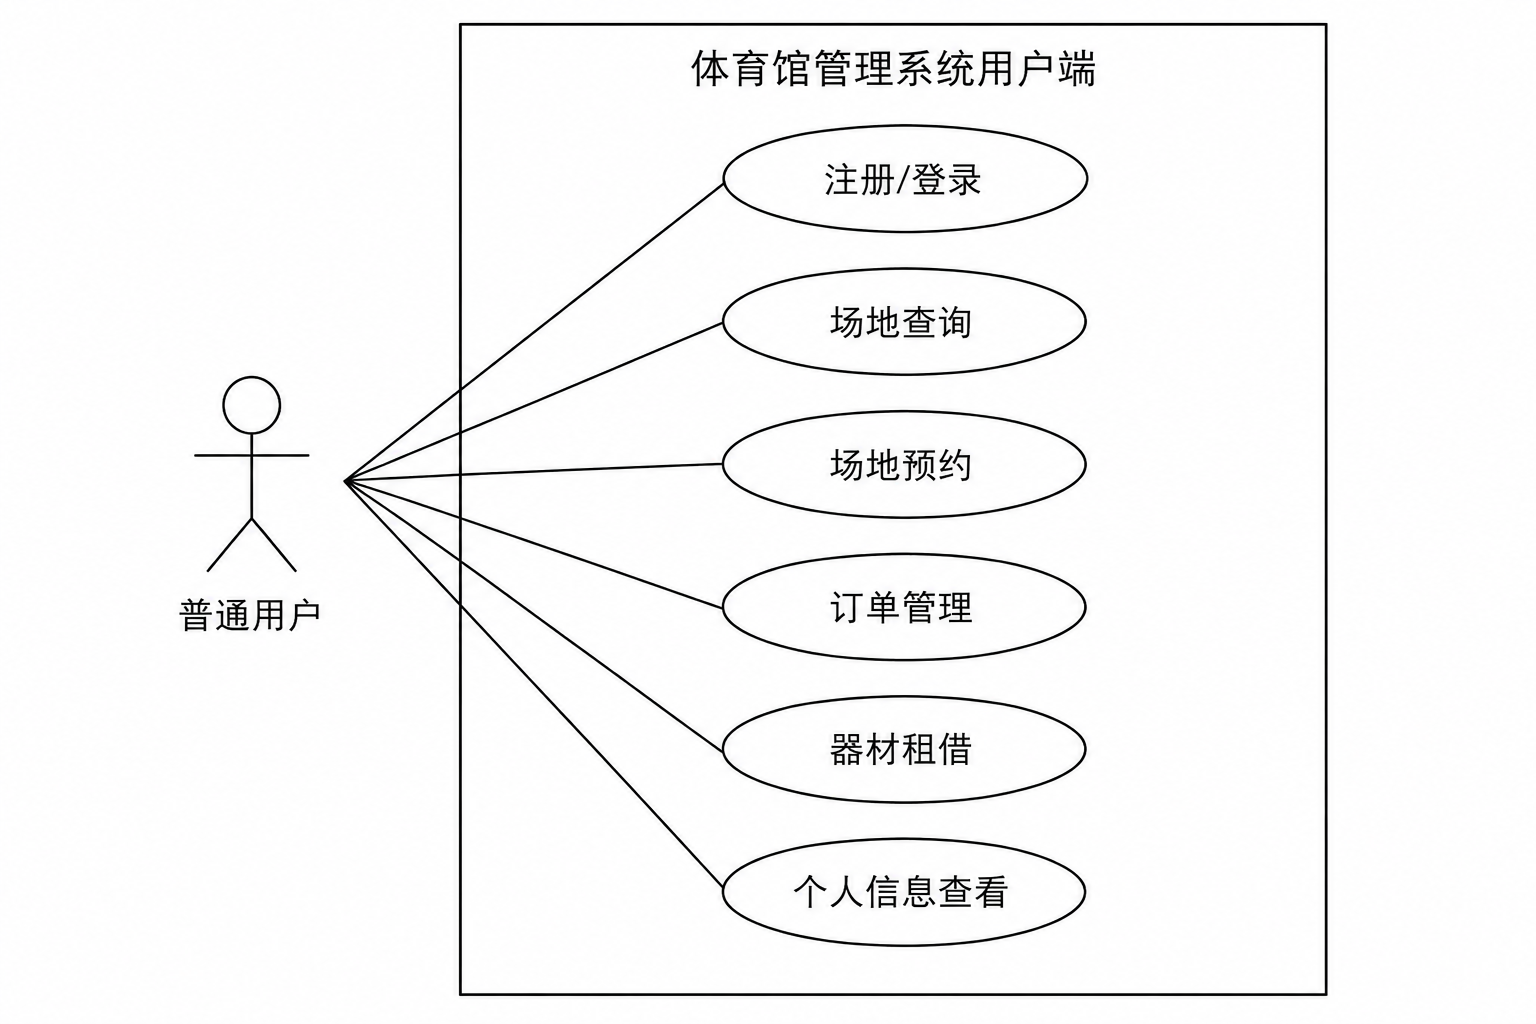
\includegraphics[width=0.78\textwidth]{img/fig3-1.png}
\caption{用户端功能用例图}
\label{fig:user-usecase-placeholder}
\end{figure}

\subsection{管理端功能需求分析}

管理端主要是对体育馆管理员进行基础数据的管理以及业务巡检工作。管理员登录后会显示后台首页的概览，即场地总数、开放场地数、订单总订单量、器材库存以及注册用户数等；管理员可以新增、修改场地信息，也可以设置场地上下架状态；管理员可以在订单管理中查看全部订单，可以按照状态筛选；管理员可以在器材管理中更新器材数量和租借单价，并对未还的设备执行归还；管理员可以查看所有的注册用户，并可以改变用户的权限。

管理端与用户端的区别在于管理员的操作会改变其它用户的可以查看或者使用的数据。场地下架之后，用户端不能继续预订这个场地；器材总数量发生变化的时候，借出的数量也要随之变动；用户的权限被提升了以后，这个账号就可以进入到后台页面了。所以管理端的需求不能只描述出“可以增删改查”，还要加上操作校验、权限控制等要求。本系统的后端管理接口使用管理员权限来限制访问，前端路由守卫可以降低出现后台页面误入的情况。

\begin{figure}[htbp]
\centering
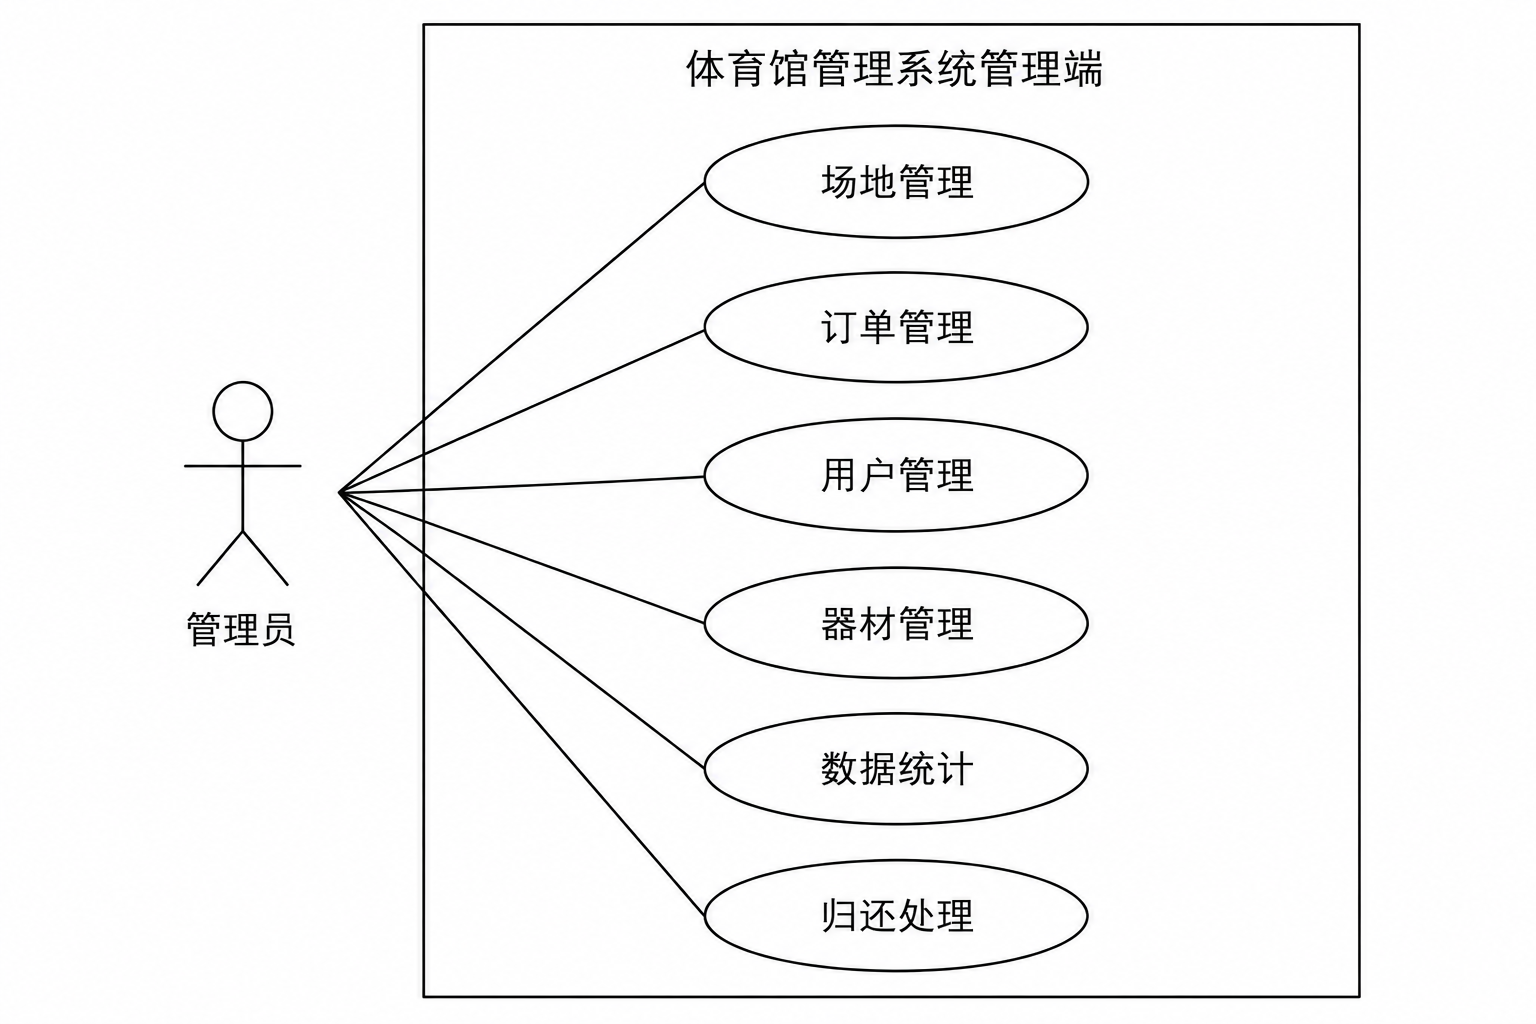
\includegraphics[width=0.78\textwidth]{img/fig3-2.png}
\caption{管理端功能用例图}
\label{fig:admin-usecase-placeholder}
\end{figure}

\section{非功能需求分析}

\subsection{性能与安全需求分析}

性能要求主要是预约高峰期。校园体育馆的访问量一般不会像大型商业平台那样大，在周末、傍晚和活动前后，场地查询、时段刷新和下单请求都会集中出现。因此系统需要保证常用列表接口可以分页返回，预约页面只请求当前场地和当前日期的时段数据，避免一次性加载过多无关的内容。订单创建接口要将冲突查询、订单写入一起放到同一个业务流程里来，以降低重复预约发生的概率。

安全需求主要包含身份认证、权限控制、输入校验这三个方面。用户登录成功之后，后端会发出 JWT，前端在之后的请求里使用 Authorization 请求头传递 token，后端拦截器从请求头中提取出用户的编号以及所扮演的角色。普通用户访问个人订单、租借记录时，应该以后端解析出来的用户编号为准，不能相信前端传入的用户编号；管理接口还需要对用户的角色进行判断，是否为 admin。场地时间、订单状态、器材数量等参数也要经过后台的二次确认才能让用户绕过前端页面直接调用接口。目前系统仍处于课程设计版本，密码存储、接口限流等安全措施还存在改善的空间，在后面的展望中也会有所提及。

\subsection{易用性与可维护性分析}

易用性看上去是个软性指标，但是对实践有着非常重要的作用。普通用户对于系统的操作没有耐心，走完一条路绕一圈，错误的提示无法看懂就放弃；管理员容忍度比较高，但是每打开一页需要点击几十次才能完成的系统，在遇到交互异常的时候效率就会受到影响。在系统方面主要的做法就是尽量减少常用的操作次数，表单失败时给出错误原因的说明，列表页提供搜索、分页等功能。

可维护性更多是针对代码的。前后端分离可以允许前后两端独立更新，修改哪个地方就有机会发现 bug，后端用控制器、服务、mapper 三个层次来组织代码，定位错误时可以直接从接口路径入手查找；前端按照页面拆成组件，公共逻辑放到 composables 中去。该种结构对以后接手开发的同学比较有利。
